\chapter{Introduction}
\label{Ch_Chapter1}


\section{Overview}

Bangladesh sits on the lower deltaic plain of the Ganges--Brahmaputra--Meghna river system, one of the largest and most hydrologically active river networks in the world. This setting, together with heavy monsoon rainfall, discharge arriving from upstream catchments, and generally low-lying terrain, leaves the country persistently exposed to flooding and water-logging. Monitoring and forecasting river water levels is, as a result, a core part of how flood risk is managed in the country.

\begin{figure}[h]
\centering
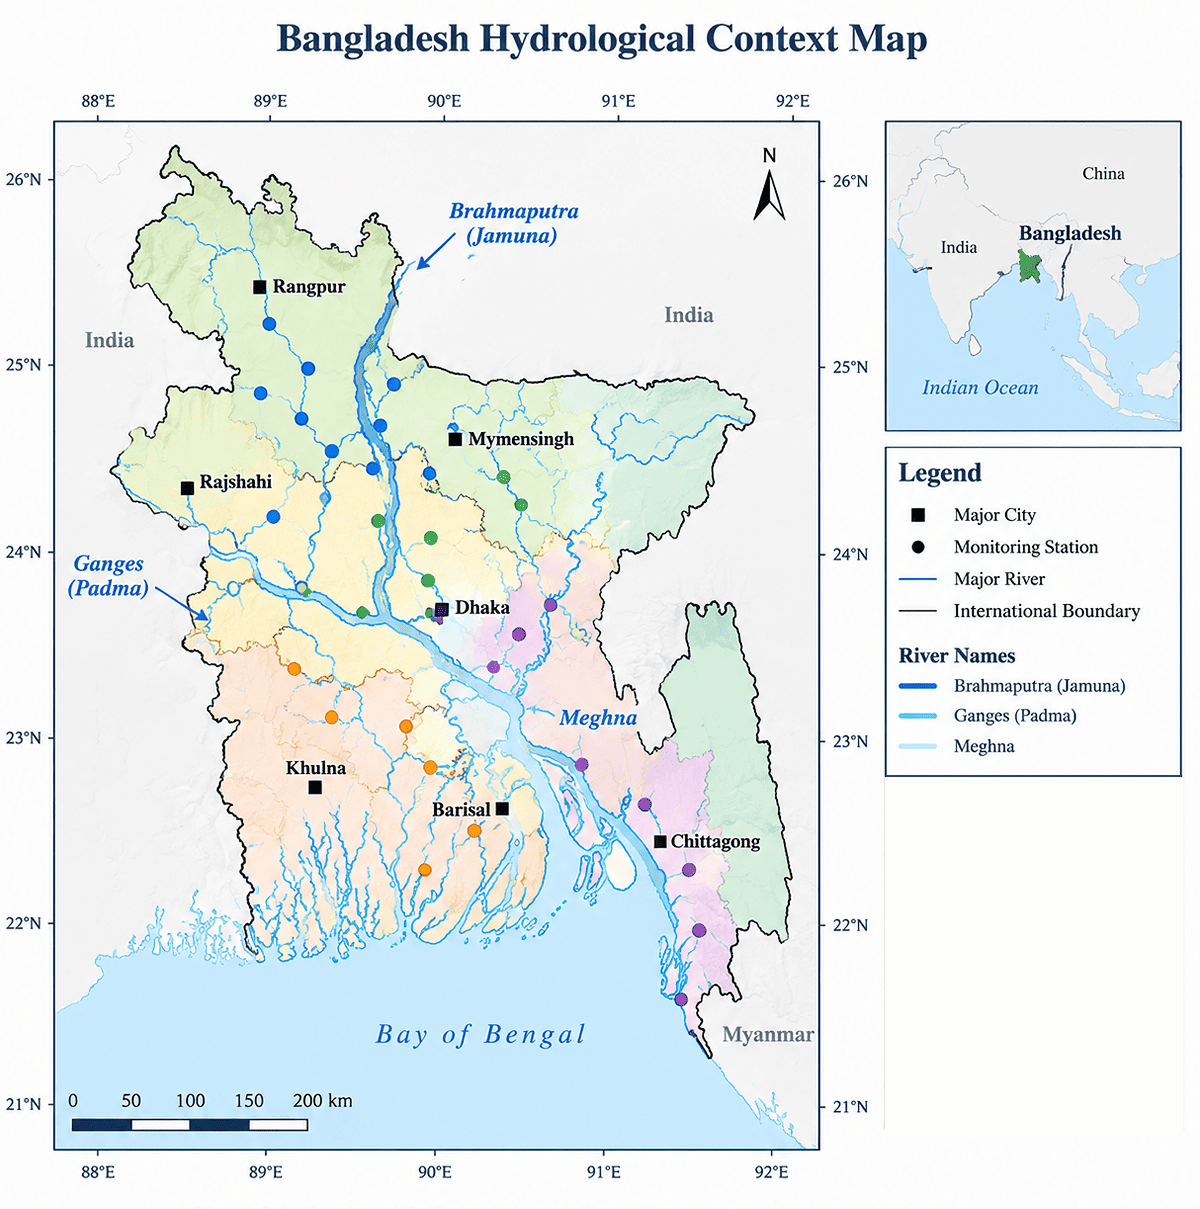
\includegraphics[width=0.85\textwidth]{figures2/fig1_1_hydro_context.png}
\caption{Bangladesh's hydrological context, showing major rivers, cities, and the study's monitoring stations.}
\label{fig:hydro-context}
\end{figure}

Figure~\ref{fig:hydro-context} gives a sense of the terrain this thesis is actually about, before the next section gets into why that terrain behaves so differently from place to place.

That risk is not distributed evenly. Rainfall, upstream discharge, the way the river network interacts with itself, and local drainage all vary from place to place, and this shows up as real differences in water-level behaviour across the country. A model built for one location will not necessarily transfer cleanly to another. This is, in effect, the starting point for the present thesis: any forecasting approach worth building for Bangladesh has to take that spatial variability seriously rather than treat it as noise.

\section{Flooding and Water-Logging in Bangladesh}

Part of what makes Bangladesh's flood problem so hard to get ahead of is that so much of it isn't generated inside the country at all. Bangladesh sits at the bottom of the Ganges--Brahmaputra--Meghna basin, and by most hydrological accounts, only a fraction of the water moving through its rivers falls as rain within its own borders --- the rest arrives from catchments upstream, across the border in India, Nepal, Bhutan, and China. In practical terms, that means a meaningful share of what shows up in a Bangladeshi river next week was already set in motion somewhere else, days earlier, by weather nobody here experienced.

The country's flood history makes this feel less abstract. In 1988, roughly 82,000 square kilometres went under water --- close to 60\% of Bangladesh --- in what's still considered a once-in-50-to-100-year event \cite{Banglapedia2023Flood}. Ten years later, 1998 went further still: more than two-thirds of the country stayed flooded, and the death toll passed 2,300 \cite{Banglapedia2023Flood,AbdullahAlam2024}. And it hasn't stopped there --- Bangladesh has seen significant flood events recur in 2004, 2007, most years between 2009 and 2014, and again in 2020, each serious enough to damage crops, roads, and household income nationally; in 2017 specifically, families in the worst-hit areas saw their annual income fall by more than a fifth \cite{AbdullahAlam2024}. None of this is distant history. It's closer to a pattern that keeps repeating, which is really the point --- this isn't a once-in-a-generation disaster this thesis is trying to help with, it's an ordinary, recurring part of life in the floodplain, and that's exactly why even a small improvement in forecast lead time or accuracy ends up mattering to a lot of people, a lot of the time.

Where the water actually causes trouble looks different depending on where you are. In rural floodplain areas, water-logging tends to follow the river fairly directly; in Bangladesh's fast-growing cities, weak drainage often turns the same rise in water level into something considerably worse. This isn't just intuition --- studies on Bangladesh back it up, showing that even neighbouring monitoring stations on the same river can behave quite differently from each other, let alone stations spread across the whole country \cite{Islam2026a,Islam2026b}. That makes sense once you think about what each part of the river is actually responding to. Upstream stations mostly react to discharge and rainfall coming down from further up the catchment. Further down, and especially around the cities, stations are shaped by a messier mix --- river flow, local rainfall, poor drainage, sometimes tidal pull as well. So there's no real basis for assuming flooding looks or behaves the same way at every station; it plainly doesn't.

None of this has gone unnoticed by researchers, to be fair. Ruma et al.\ forecast water levels across a wide network of Bangladeshi river stations using an optimized LSTM \cite{Ruma2023}. Others came at it from the meteorological side, pairing climatic variables with machine learning or deep learning to predict flooding \cite{Rakin2023,Rajab2023}, while more recent work has zeroed in on river discharge and broader hydrological modelling specifically in the Old Brahmaputra basin \cite{Islam2026a,Islam2026b}. Put together, these studies build a pretty convincing case that data-driven forecasting can work here --- but they also keep landing, sometimes explicitly, on the same conclusion: individual stations have their own character, and averaging that away loses something real.

\section{Importance of Water-Level Forecasting}

Given all this, forecasting that is reliable, timely, and sensitive to where a station actually sits in the river network is important for flood preparedness, early warning, and reducing disaster risk more generally. Different lead times are useful for different kinds of decisions: a forecast a few hours ahead supports an immediate response, while a forecast weeks ahead is more useful for planning.

The lead time itself matters a great deal, because the further out a forecast reaches, the harder it generally becomes to get right. Even so, machine-learning and deep-learning models have shown real potential for multi-step forecasting that extends to several days or weeks ahead \cite{Islam2026a,Ruma2023}. Encoder--Decoder architectures have specifically been explored for multi-step-ahead flood forecasting and offer a natural way of producing a whole sequence of future values rather than a single prediction at a time \cite{Kao2020,Cui2022}, though it is worth noting that both of these studies were evaluated at horizons of hours rather than days --- a distinction this thesis returns to in Chapter 2.

A framework that can forecast across several horizons at once, from the near-term to the longer-term, therefore offers a more complete picture of what is likely to happen than one built around a single lead time alone.

\section{Problem Statement}

Most of the water-level and flood-forecasting work done in Bangladesh so far leans on one particular type of data, or a fairly narrow combination of variables. Ruma et al. worked from water-level records alone \cite{Ruma2023}; more recent work on river discharge has largely done the same with discharge \cite{Islam2026a}; and a separate strand of research has approached flood prediction almost entirely through climatic and meteorological information \cite{Rakin2023,Rajab2023,HemelSakib2024}. Each of these lines of work is useful in its own right, but none of them really grapples with what happens when discharge, water level, and weather variables are brought together across a large and hydrologically varied network of stations.

There is a second, related issue: where the data actually comes from. Stations in different parts of a river network can behave quite differently from one another statistically, and a single model trained on pooled data from all of them may end up representing none of them particularly well. Bangladeshi hydrological studies have already applied machine-learning and deep-learning models across multiple sites, but almost always under the assumption that the data can first be brought together in one place \cite{Islam2026a,Islam2026b,Ruma2023}.

Federated learning offers a different way of thinking about this. Rather than pooling data, distributed clients train collaboratively while keeping their raw data where it is. McMahan et al.'s Federated Averaging (FedAvg) algorithm was the first to show, convincingly, how model updates from many separate clients could be combined into a single shared model without ever collecting their underlying data centrally \cite{McMahan2017}. The catch is that this works best when client data are reasonably similar to one another; when they are not --- when they are, in the technical sense, non-independent and identically distributed, or non-IID --- standard federated learning can struggle \cite{Zhu2021,Chen2025}. That kind of heterogeneity is exactly what one would expect across stations that sit in different parts of a river system.

Clustered Federated Learning (CFL) is one response to that problem: rather than forcing every client into a single shared model, clients that look similar to one another are grouped together and trained as a cluster. Work in this area has shown that this kind of grouping can produce more specialized, better-performing models than either a single global model or fully isolated local ones \cite{Ghosh2021,Harshvardhan2022,BenAli2026}. What is missing is any application of this idea to a real, multi-station, multi-horizon water-level forecasting problem in Bangladesh.

There is also a more practical concern. A forecast is only as useful as the trust placed in it, and that trust is harder to build when a model cannot explain why it predicted what it predicted. Explainable AI methods address this gap directly. SHAP, in particular, has become a widely used and theoretically well-grounded way of attributing a model's prediction to its individual inputs \cite{Lundberg2017}, and it has already been applied usefully in flood and water-level prediction \cite{Huang2024,Khorrami2025}.

Put together, the central problem this thesis addresses is how to forecast water levels accurately, across multiple horizons, for a network of Bangladeshi monitoring stations that are hydrologically quite different from one another, without needing to centralize their raw data, and while still being able to explain what is driving the model's predictions.

\section{Research Motivation}

Three strands of existing work, taken together, motivate this study.

The first concerns architecture. Deep sequence models, and LSTM in particular, have repeatedly proven effective for hydrological time series, including multi-step-ahead prediction \cite{Ruma2023,Kao2020,Cui2022}. Encoder--Decoder LSTM designs are especially well suited to this, since they naturally produce a sequence of future values rather than a single one \cite{Kao2020,Cui2022}, and more recent Seq2Seq and residual-LSTM variants confirm that this general approach remains relevant \cite{Lim2025,Yuan2023}. This is the main reason an Encoder--Decoder LSTM is chosen as the core forecasting architecture here.

The second strand is about how training happens rather than what is being trained. Federated learning makes it possible to train collaboratively while leaving raw observations where they are \cite{McMahan2017}, but non-IID data among clients is a genuine obstacle to doing this well \cite{Zhu2021,Chen2025}. Clustering clients before training, rather than after something has already gone wrong, is one practical way around this \cite{Ghosh2021,Harshvardhan2022,BenAli2026}, and there is at least one early example of federated learning being applied to hydrological forecasting specifically \cite{Amanzholova2026}, which suggests the idea is workable, even if not yet explored at any scale.

The third strand concerns trust and interpretability. As machine-learning models get folded into decisions that matter --- flood warnings among them --- being able to say why a model predicted what it did becomes as important as the prediction itself. SHAP provides a principled way of doing this \cite{Lundberg2017}, and its use in flood-related modelling has already shown that it can surface genuinely useful relationships between hydrometeorological inputs and model outputs \cite{Huang2024,Khorrami2025,Parasar2025}.

None of these three strands, on their own, is new. What has not been done is bringing them together --- multivariate hydrometeorological inputs, an Encoder--Decoder architecture, cluster-aware federated training, forecasting across multiple horizons, and interpretability --- into a single framework built for the Bangladeshi context.

\section{Research Gap}

Progress has clearly been made on each front separately: Bangladesh-specific forecasting, multi-step deep learning, federated learning, clustered federated learning, and explainable hydrological modelling all have a reasonably developed literature behind them. What they do not have, so far, is much overlap.

Bangladesh-focused studies have shown that machine learning and deep learning can forecast water level, discharge, and flood occurrence reasonably well \cite{Islam2026a,Islam2026b,Ruma2023,Rakin2023,Rajab2023,HemelSakib2024}. Separately, work on multi-step forecasting has established that Encoder--Decoder and Seq2Seq architectures are a sound way of generating forecasts across several future time steps \cite{Kao2020,Cui2022,Lim2025,Yuan2023}. Federated learning research has tackled decentralized training and the non-IID problem in general terms \cite{McMahan2017,Zhu2021,Chen2025}, and clustered federated learning has offered a specific mechanism --- grouping similar clients --- for handling that heterogeneity \cite{Ghosh2021,Harshvardhan2022,BenAli2026}. And SHAP-based explainability has already found its way into flood and hydrological modelling \cite{Lundberg2017,Huang2024,Khorrami2025}.

But no study identified in this review brings these threads together: multi-horizon water-level forecasting, across a large and multivariate network of Bangladeshi stations, using a cluster-aware federated architecture, with SHAP-based interpretation, and checked against an external reference such as the Flood Forecasting and Warning Centre (FFWC).

That is the gap this thesis sets out to close, with a Clustered Federated Learning framework built around an Encoder--Decoder LSTM (CFL-EDLSTM) for multi-horizon water-level forecasting in Bangladesh.

\section{Aim of the Study}

The aim of this study is to design, build, and evaluate a Clustered Federated Learning framework based on an Encoder--Decoder LSTM (CFL-EDLSTM), for privacy-preserving, multi-horizon, and interpretable water-level forecasting across 25 hydrologically diverse monitoring stations along the Brahmaputra River system in Bangladesh.

Alongside the forecasting framework itself, the study also demonstrates how these outputs might actually be presented to someone using them, through a web-based visualization platform. The platform gives station-level forecast information and lets a user compare CFL-EDLSTM's predictions against water-level information published by the Flood Forecasting and Warning Centre (FFWC), used here as an external point of comparison rather than as ground truth.

\section{Research Objectives}

The objectives of this study are:

\begin{enumerate}
    \item To develop a clustering strategy that groups 25 hydrologically diverse Bangladeshi monitoring stations within the Brahmaputra River system into four meaningful clusters: Upstream, Middle, Downstream, and Urban.

    \item To develop an Encoder--Decoder LSTM (EDLSTM) architecture capable of multivariate, multi-horizon water-level forecasting across seven lead times, ranging from 3 hours to 15 days.

    \item To integrate the EDLSTM architecture within a Clustered Federated Learning (CFL) framework using Federated Averaging (FedAvg) for cluster-specific parameter aggregation without centralizing raw station-level data.

    \item To benchmark the proposed CFL-EDLSTM framework against four baseline architectures --- Vanilla LSTM, GRU, XGBoost, and TCN --- across different station clusters and forecast horizons.

    \item To apply SHAP-based interpretability to the trained models in order to identify and rank the hydrometeorological variables contributing to model predictions.

    \item To develop a web-based visualization platform that presents CFL-EDLSTM forecasts and compares them against water-level information published by the Flood Forecasting and Warning Centre (FFWC) as an external reference.
\end{enumerate}

\section{Research Questions}

This study is guided by the following questions:

\begin{enumerate}
    \item How can 25 hydrologically diverse monitoring stations within the Brahmaputra River system in Bangladesh be grouped into clusters that are meaningful for federated training?

    \item How effectively can an Encoder--Decoder LSTM architecture forecast water levels across horizons ranging from short-term (3 hours) to long-term (15 days)?

    \item How well does the proposed Clustered Federated Learning approach handle heterogeneity among the four station clusters while keeping station-level data private?

    \item How does the proposed CFL-EDLSTM framework perform relative to Vanilla LSTM, GRU, XGBoost, and TCN baselines across different clusters and lead times?

    \item Which input variables --- water level, discharge, rainfall, temperature, or evaporation --- contribute most to model predictions according to SHAP, and do those contributions make hydrological sense?

    \item How closely do CFL-EDLSTM's forecasts, as shown through the web-based visualization platform, align with water-level information published by FFWC, used here as an external point of comparison rather than as ground truth?
\end{enumerate}

\section{Scope of the Study}

This study is built around 25 selected monitoring stations within the Brahmaputra River system in Bangladesh, grouped into four clusters --- Upstream, Middle, Downstream, and Urban --- based on their hydrological characteristics and where they sit within the river network.

Five variables are used: water level, discharge, rainfall, temperature, and evaporation, with water level as the target. Forecasts are generated across seven lead times: 3 hours, 6 hours, 12 hours, 1 day, 3 days, 7 days, and 15 days.

CFL-EDLSTM is compared against four baseline architectures --- Vanilla LSTM, GRU, XGBoost, and TCN --- reflecting the broader set of modelling approaches identified in recent flood-prediction literature \cite{Aghenda2025}, and interpreted using SHAP \cite{Lundberg2017,Huang2024}.

What this study does not attempt is real-time operational deployment, a mobile application, or forecasting of anything beyond water level. The web-based visualization interface is built to demonstrate and validate the framework, not to serve as an operational early-warning system in its own right.

\section{Contributions of the Study}

This thesis makes the following contributions:

\begin{enumerate}
    \item A clustering strategy that groups 25 monitoring stations within the Brahmaputra River system into four meaningful federated client groups: Upstream, Middle, Downstream, and Urban.

    \item A Clustered Federated Learning framework based on an Encoder--Decoder LSTM (CFL-EDLSTM), for privacy-preserving, multivariate, multi-horizon water-level forecasting across heterogeneous monitoring stations.

    \item A comparative evaluation of CFL-EDLSTM against four established baseline architectures across multiple station clusters and seven forecast horizons.

    \item A SHAP-based interpretability analysis identifying which hydrometeorological variables matter most, and where, across the different station clusters.

    \item A web-based visualization and comparison platform that presents CFL-EDLSTM forecasts alongside FFWC water-level information, showing how the framework's results might practically be used.
\end{enumerate}

\section{Overview of the Proposed Framework}

At a high level, CFL-EDLSTM combines a sequence-to-sequence Encoder--Decoder LSTM \cite{Kao2020,Cui2022} with a Clustered Federated Learning training procedure. The federated part of this borrows directly from McMahan et al.'s original idea: model updates travel from distributed clients to a central point of aggregation, but the raw data behind those updates never does \cite{McMahan2017}.

In this framework, the 25 monitoring stations are first grouped into four clusters based on their hydrological characteristics and position within the river network. Each station then acts as a local client within its cluster, training the EDLSTM model on its own multivariate data. Rather than being sent anywhere, that data stays local; only the resulting model parameters are shared, and Federated Averaging (FedAvg) is used to combine them into a single model per cluster \cite{McMahan2017}.

This is a deliberate departure from a conventional federated setup, where all clients would ultimately contribute to one shared global model. Here, each cluster keeps its own model. The reasoning follows directly from the literature reviewed above: non-IID data across clients can genuinely hurt standard federated learning \cite{Zhu2021,Chen2025}, whereas clustering clients with similar characteristics tends to produce better, more specialized models \cite{Ghosh2021,Harshvardhan2022,BenAli2026}.

Once trained, the four cluster models generate water-level forecasts across all seven horizons. SHAP is then applied to interpret those forecasts and see which variables are actually driving them \cite{Lundberg2017,Huang2024,Khorrami2025}. Finally, everything is made accessible through an interactive web-based map, with a separate section for comparing the model's output against FFWC's published water-level information.

The full implementation and experimental design behind this framework are described in Chapter 3.

\section{Organization of the Thesis}

The rest of this thesis is organized into four chapters.

\textbf{Chapter 2} reviews the literature underpinning this study --- Bangladesh-specific flood and water-level forecasting, hydrological and meteorological time-series modelling, machine learning and deep learning, Encoder--Decoder LSTM architectures, multi-horizon forecasting, federated learning, clustered federated learning, and explainable AI --- and closes with a critical synthesis that identifies the specific gap this thesis addresses.

\textbf{Chapter 3} sets out the methodology: the study area, monitoring stations, data sources, input and target variables, preprocessing, the station-clustering strategy, the forecasting setup, the proposed CFL-EDLSTM architecture and its federated aggregation procedure, the baseline models, the multi-horizon evaluation design, the performance metrics, the SHAP analysis, and the web-based visualization platform.

\textbf{Chapter 4}, once experiments have been run, will present and discuss the results --- the clustering outcomes, CFL-EDLSTM's overall performance, its comparison against the baselines, its performance across different horizons and clusters, the SHAP findings, station-level visualizations, and the comparison against FFWC.

\textbf{Chapter 5} will close the thesis with a summary of what was found, how well the objectives were met, the study's contributions and limitations, and directions for future work.


